\addcontentsline{toc}{chapter}{Introduction}

Laure Bruhat a entamé depuis plus de deux ans une thèse portant notamment sur la séparation des paires de Cooper intriquées dans une cavité micro-ondes et le transport quantique. Pour ce faire, elle a mis en place une expérience dans un cryostat à dilution sèche, fourni par CryoConcept.
\par
\begin{figure}[h]
    \begin{center}
        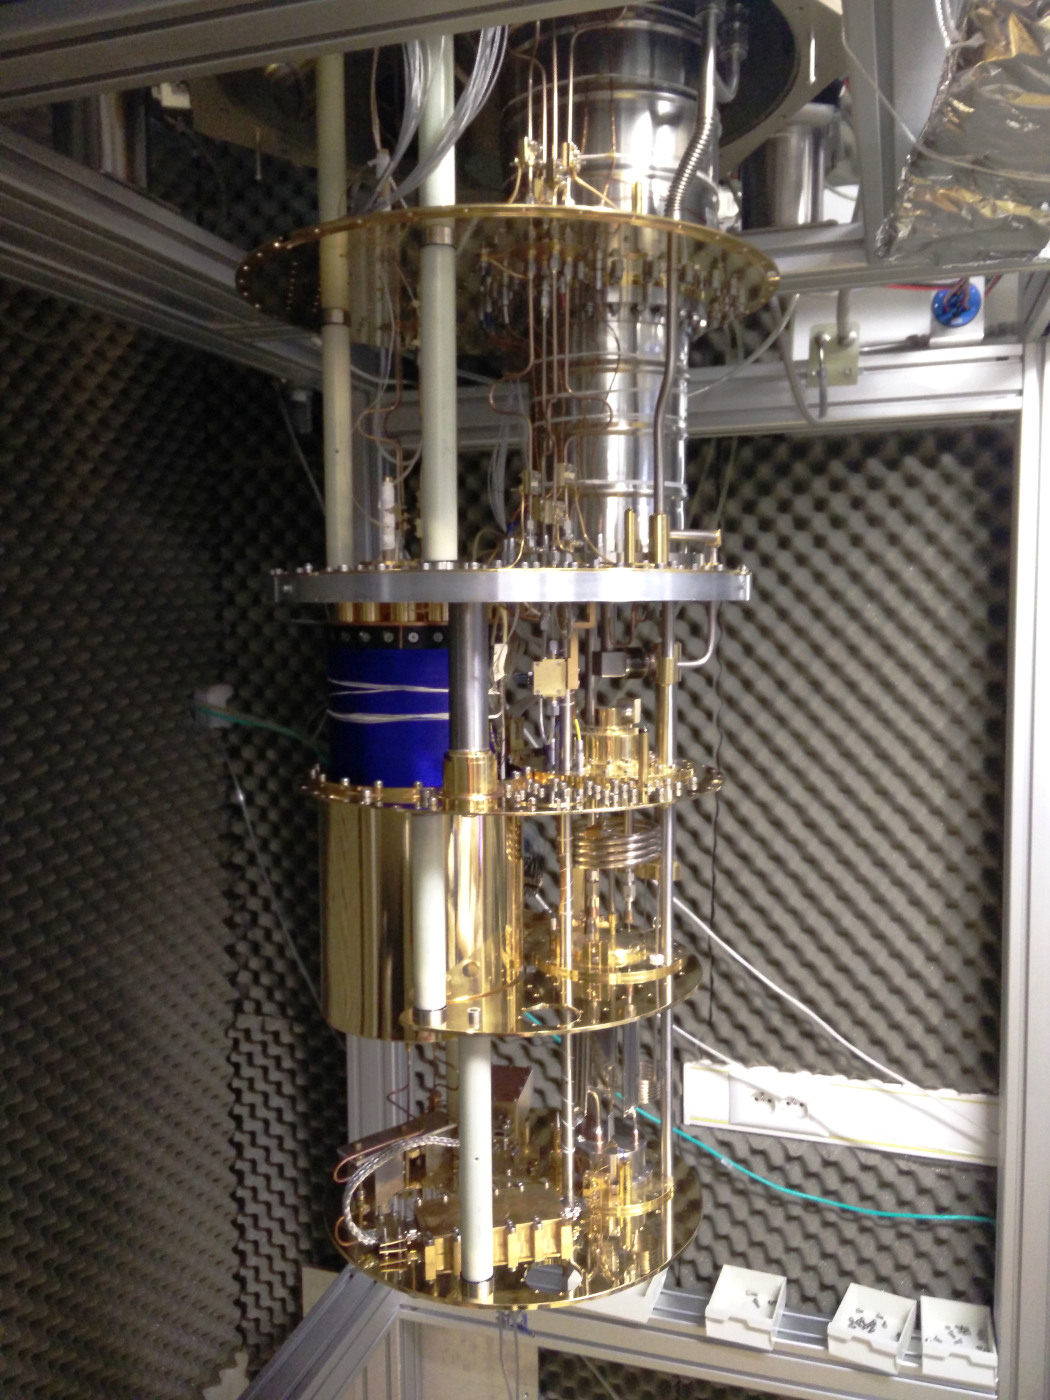
\includegraphics[height=0.7\textwidth]{Images/Global.jpg}
        \caption*{Le cryostat ouvert avec la bobine (bleue)}
        \label{photo_separateur_nanotube}
    \end{center}
\end{figure}


Ce cryostat étant "spacieux", Takis Kontos et Laure Bruhat ont décidé d'y rajouter une expérience. Celle-ci serait placée au sein d'un champ magnétique, généré par une bobine installée dans le cryostat. Cette expérience pourra donc permettre d'étudier l'influence du champ magnétique (~700mT) sur la séparation des paires de Cooper.
\par

Mon travail consiste donc à comprendre l'ensemble du fonctionnement du cryostat, et à câbler la seconde expérience, de la fabrication des câbles à leur caractérisation et leur mise en place dans le cryostat. Il consiste aussi à mettre à froid pour les divers tests du cryostat après la mise en place de la bobine.
